\documentclass[border=10pt]{standalone}
\usepackage{tikz}
\usetikzlibrary{3d, arrows.meta, calc, positioning}

\begin{document}

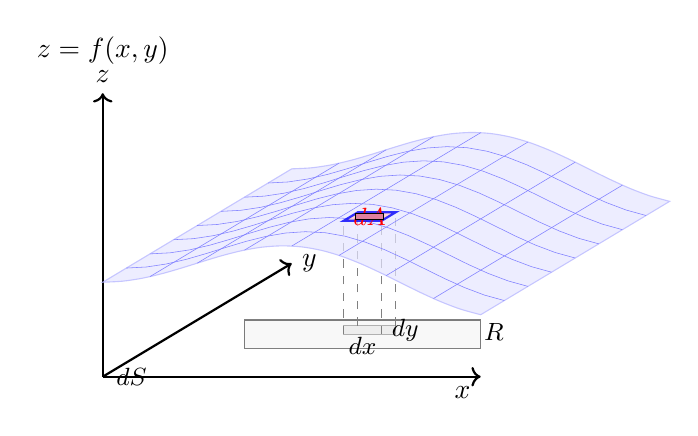
\begin{tikzpicture}[
    scale=1.2,
    x={(1cm,0cm)}, y={(0.5cm,0.3cm)}, z={(0cm,1cm)},
    axis/.style={->, thick},
    surface/.style={blue!30, fill=blue!10, opacity=0.7},
    grid/.style={blue!50, very thin},
    dA/.style={draw=blue, thick, fill=red!20, opacity=0.8},
    dxdy/.style={draw=gray, fill=gray!20, opacity=0.6},
    label/.style={font=\small, inner sep=1pt},
    projection/.style={dashed, gray}
]

% Axes
\draw[axis] (0,0,0) -- (4,0,0) node[below left] {$x$};
\draw[axis] (0,0,0) -- (0,4,0) node[right] {$y$};
\draw[axis] (0,0,0) -- (0,0,3) node[above] {$z$};

% Label z = f(x,y)
\node[above] at (0,0,3.2) {$z = f(x,y)$};

% Region R in xy-plane
\draw[fill=gray!10, opacity=0.5] (1,1,0) rectangle (3,2,0);
\node[label, below right] at (3,2,0) {$R$};

% dx and dy elements
\draw[dxdy] (1.8,1.5,0) rectangle ++(0.4,0.3,0);
\node[label, below] at (2.0,1.5,0) {$dx$};
\node[label, right] at (2.2,1.65,0) {$dy$};

% Projection lines to surface
\draw[projection] (1.8,1.5,0) -- (1.8,1.5,1.2);
\draw[projection] (2.2,1.5,0) -- (2.2,1.5,1.2);
\draw[projection] (1.8,1.8,0) -- (1.8,1.8,1.2);
\draw[projection] (2.2,1.8,0) -- (2.2,1.8,1.2);

% Surface z = f(x,y) - approximated as a curved plane
\draw[surface, smooth] 
    plot[domain=0:4, samples=20] (\x,0,{0.5*sin(\x r)*sin(0.5*\x r)+1}) --
    plot[domain=4:0, samples=20] (4,\x,{0.5*sin(4 r)*sin(0.5*4 r)+1}) --
    plot[domain=4:0, samples=20] (\x,4,{0.5*sin(\x r)*sin(0.5*\x r)+1}) --
    plot[domain=4:0, samples=20] (0,\x,{0.5*sin(0 r)*sin(0.5*0 r)+1}) -- cycle;

% Add grid on surface
\foreach \i in {0.5,1,...,3.5} {
    \draw[grid] plot[domain=0:4, samples=20] (\i,\x,{0.5*sin(\i r)*sin(0.5*\i r)+1});
    \draw[grid] plot[domain=0:4, samples=20] (\x,\i,{0.5*sin(\x r)*sin(0.5*\x r)+1});
}

% dA element on surface
\draw[dA] (1.8,1.5,1.2) -- (2.2,1.5,1.2) -- (2.2,1.8,1.2) -- (1.8,1.8,1.2) -- cycle;
\node[label, red] at (2.0,1.65,1.2) {$dA$};

% Small purple rectangle inside dA for emphasis
\draw[fill=purple!50] (1.9,1.55,1.2) rectangle (2.1,1.75,1.2);

% Label dS near x-axis
\node[label, left] at (0.5,0,0) {$dS$};

\end{tikzpicture}

\end{document}